\documentclass[12pt]{article}

\input sketch.sty

%Personnages :
\def\henry{Henry}
\def\assoResp{Responsable de l'association}
\def\compDir{Directrice de l'entreprise}
\def\maman{Maman}
\def\ami{Ami}
\def\fille{Belle fille}
\def\mentor{Mentor}
\def\collOut{Collègue out}
\def\collIn{Collègue in}

\title{\textsf{XOR (eXclusive OR)}}
\author{Groupe de jeunes de \\ l'Eglise Evangélique du Lac}
\date{Fête de Noël \\ Samedi 22 décembre 2012}

\begin{document}

\maketitle

	\begin{figure}[htb]
	\centering
	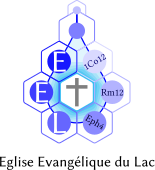
\includegraphics[width=5cm]{Figures/logoEEL11.pdf}
	\end{figure}

\newpage

\begin{center}
\textit{A Nicolas}
\end{center}

\vfill

\begin{abstract}
Cette année, je devais choisir entre un stage avec les GBU
(Groupes Bibliques Universitaires) et un doctorat de physique.
Ce sketch s'inspire de ce choix difficile.
Son message est simple : d'abord évangéliser nos proches,
nos amis et nos collègues.
\end{abstract}

\setcounter{tocdepth}{2}
\tableofcontents

\vfill

\newpage

\input Sections/prep.tex

\newpage

\section{Dialogues}

	\input Sections/dialogues_intro.tex
	\input Sections/dialogues_disc.tex
	\input Sections/dialogues_evang.tex
	
\newpage
	
\input Sections/insp.tex

\vfill

\begin{center}
Compilé le \today{} par \LaTeX{}.
\end{center}

\end{document}